\documentclass[final]{beamer}
\RequirePackage{beamertransparentboxes}
\RequirePackage{pgfpages}

% \documentclass[handout,final]{article}
% \RequirePackage{beamerarticle}

\setbeamerfont{note page}{size=\scriptsize}
\addtobeamertemplate{note page}{\setbeamerfont{itemize/enumerate subbody}{size=\scriptsize}\setlength{\parindent}{0pt}\setlength{\parskip}{.7em}}{\par}

\mode<handout>{%
    \pgfpagesuselayout{2 on 1}[a4paper] 
    \setbeameroption{show notes on second screen=bottom}
}

\usetheme{Warsaw}

\RequirePackage[utf8]{inputenc}
\DeclareUnicodeCharacter{00A0}{ }

\RequirePackage{color}
\definecolor{ao(english)}{rgb}{0.0, 0.5, 0.0}
\definecolor{blue(pigment)}{rgb}{0.2, 0.2, 0.6}
\definecolor{egyptianblue}{rgb}{0.06, 0.2, 0.65}

\RequirePackage{listings}
\lstset{
    basicstyle=\scriptsize
}

\RequirePackage{graphicx}

\RequirePackage{amsthm}
\RequirePackage{amsmath}
\RequirePackage{amsfonts}
\RequirePackage{soul}
\RequirePackage{xspace}
\RequirePackage{bussproofs}
\RequirePackage[customcolors]{hf-tikz}

\RequirePackage{tikz}

\RequirePackage{multicol}
\RequirePackage{lipsum}
\RequirePackage{textpos}

\setlength{\parindent}{0pt}
\setlength{\parskip}{.7em}

\RequirePackage{polski}

\uselanguage{polski}
\languagepath{polski}
\deftranslation[to=polski]{Definition}{Definicja}

\logo{\includegraphics[height=.3\textheight]{logo.png}}

\title{Kombinatoryczne interpretacje rekurencji holonomicznych}
\author[Bartłomiej Puget (TCS UJ)]{Bartłomiej Puget\\Promotor: dr Katarzyna Grygiel}
\institute{Theoretical Computer Science\\Jagiellonian University}

\date{Kraków, 19 maja 2021}

\makeatletter
\def\th@bluetheorem{%
    \normalfont % body font
    \setbeamercolor{block title example}{bg=blue(pigment),fg=white}
    \setbeamercolor{block body example}{bg=blue(pigment)!20,fg=black}
    \setbeamercolor{item}{fg=blue(pigment)}
    \def\inserttheoremblockenv{exampleblock}
}
\def\th@greentheorem{%
    \normalfont % body font
    \setbeamercolor{block title example}{bg=ao(english),fg=white}
    \setbeamercolor{block body example}{bg=ao(english)!20,fg=black}
    \setbeamercolor{item}{fg=ao(english)}
    \def\inserttheoremblockenv{exampleblock}
}
\makeatother

\theoremstyle{bluetheorem}
\newtheorem{mytheorem}{Definicja}[section]

\theoremstyle{bluetheorem}
\newtheorem{mydefinition}[mytheorem]{Definicja}
\newtheorem{myproductions}[mytheorem]{Produkcje}

\theoremstyle{greentheorem}
\newtheorem{myexample}[mytheorem]{Przykład}

\begin{document}
\maketitle

\section{Wstęp}

\begin{frame}{Rekurencje holonomiczne}
    \begin{mydefinition}
        Ciąg \((a_n)_{n=0}^\infty\) jest P-rekurencyjny (holonomiczny) wtedy i tylko wtedy, gdy istnieje dla niego rekurencja holonomiczna, tj.:
        \[\exists_{r \in \mathbb{N}} \exists {p_0, \ldots, p_r : \text{ poly }}\forall_{n \in \mathbb{N}}:\]
        \[p_0(n) a_n + p_1(n) a_{n + 1} + \ldots + p_r(n) a_{n + r} = 0\]
    \end{mydefinition}

    \begin{myexample}
        \(a_n = \frac{5 n - 3}{3 n + 5}\) jest holonomiczny, gdyż zachodzi:
        \[(3n + 5) (5n + 2) a_n - (5n - 3)(3n + 8) a_{n + 1} = 0\]
    \end{myexample}
\end{frame}

\begin{frame}{Rekurencje holonomiczne (równoważnie)}
    \begin{mydefinition}
        Ciąg \((a_n)_{n=0}^\infty\) jest P-rekurencyjny (holonomiczny) wtedy i tylko wtedy, gdy istnieje dla niego funkcja tworząca:
        \[p_0(z) C(z) + p_1(z) C'(z) + \ldots + p_r(z) C^{(r - 1)}(z) = b(z)\]
        dla pewnych:\\
        \(r \in \mathbb{N}\)\\
        \(b, p_0, \ldots, p_r : \text{ poly }\)
    \end{mydefinition}
\end{frame}

\begin{frame}{Rekurencje holonomiczne}
    \begin{myexample}
        \begin{center}
            \includegraphics[width=.5\textwidth]{catalan_image.png}
        \end{center}
        \[C(z) = z + 2 z C(z) + z C^2(z)\]
        \[(n + 2) C_{n + 1} = 2(2n + 1) C_n \]
    \end{myexample}
\end{frame}

\begin{frame}{Interpretacje kombinatoryczne}
    \begin{myexample}
        \[(n + 2) C_{n + 1} = 2 (2n + 1) C_{n}\]

        \begin{center}
            \includegraphics{catalan_interpretation.png}
        \end{center}
    \end{myexample}
\end{frame}

\section{Problem}

\begin{frame}{Drzewa termów lambda w notacji de Bruijna}
    \begin{columns}
        \column{.5\textwidth}
        \begin{mydefinition}
            \begin{itemize}
                \item \(\forall n \in \mathbb{N}: n \text{ jest termem}\)
                \item \(P \text{ jest termem} \implies \lambda P \text{ jest termem}\)
                \item \(P, Q \text{ są termami} \implies P @ Q \text{ jest termem}\)
            \end{itemize}
        \end{mydefinition}

        \column{.5\textwidth}
        \begin{myexample}
            \begin{center}
                \includegraphics{lambda_001.png}
            \end{center}
        \end{myexample}
    \end{columns}
\end{frame}

\begin{frame}{Drzewa termów lambda w notacji de Bruijna}
    \begin{myexample}
        \begin{columns}
            \column{.475\textwidth}
            \begin{center}
                \includegraphics[height=\textwidth]{example_007.png}
            \end{center}
            \column{.05\textwidth}
            \begin{center}
                    \raisebox{.25\textwidth}{$\equiv$}
            \end{center}
            \column{.475\textwidth}
            \begin{center}
                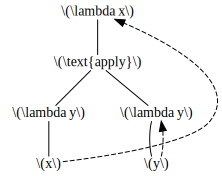
\includegraphics[height=\textwidth]{example.png}
            \end{center}
        \end{columns}
    \end{myexample}
\end{frame}

\begin{frame}{Rekurencja holonomiczna}
    \begin{columns}
        \column{.6\textwidth}
        \begin{mydefinition}
            \[\begin{array}{rcl}
                         0 &=& (n + 1)C_n\\
                           &-& (4n - 1)C_{n-1}\\
                           &+& (2n - 1)C_{n-2}\\
                           &+& C_{n-3}\\
                           &+& (n - 4)C_{n-4}
            \end{array}\]
        \end{mydefinition}

        \column{.4\textwidth}
        \begin{myexample}
            \begin{center}
                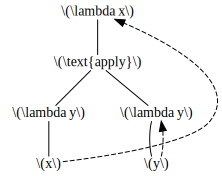
\includegraphics[width=.8\textwidth]{example.png}
            \end{center}
        \end{myexample}
    \end{columns}
\end{frame}

\section{Podejścia do problemu}

\begin{frame}{Różnicowanie wag wierzchołków}
    \begin{mydefinition}
        \[\begin{array}{rcl}
                0 &=& (n + a)C_{n} \\
                  &-& (2n - 3l + 2a)C_{n-l} \\
                  &+& (n - 3l + a)C_{n-2l} \\
                  &-& (4n - 6o - 2a)C_{n-o-a} \\
                  &+& (4n - 6o - 2s - 2a)C_{n-o-s-a} \\
                  &-& (2n - 2s + 2a)C_{n-s} \\
                  &+& (4n - 4s - 6l + 4a)C_{n-s-l} \\
                  &-& (2n - 2s - 6l + 2a)C_{n-s-2l} \\
                  &+& (n - 2s + a)C_{n-2s} \\
                  &-& (2n - 4s - 3l + 2a)C_{n-2s-l} \\
                  &+& (n - 2s - 3l + a)C_{n-2s-2l}
        \end{array}\]
    \end{mydefinition}
\end{frame}

\begin{frame}{Przyrównanie do rekurencji intuicyjnej}
    \begin{mydefinition}
        \small
        \[\begin{array}{rcl}
                C_n &=& 1 + C_{n - 1} + \sum_{k=1}^{n-2}C_k*C_{n - k - 1} \\
                (4n - 1)C_{n - 1} &=& (n + 1)C_n + (2n - 1)C_{n - 2} + C_{n - 3} + (n - 4)C_{n - 4}
        \end{array}\]
    \end{mydefinition}
\end{frame}

\begin{frame}{Iteracyjne drążenie tematu}
    \begin{mydefinition}
        \[\begin{array}{rcl}
            L &=& zaL^2 + zlL + uS\\
            S &=& zo + zsS
        \end{array}\]
    \end{mydefinition}

    \begin{mydefinition}
        \[\begin{array}{rcl}
                0 &=& (n + 1)C_n\\
                  &+& (-2ns - (2n - 1)l)C_{n - 1}\\
                  &+& ((n-1) s^2 + 2(2n-3)ls + (n-2)l^2 -4(n-2)aou)C_{n - 2}\\
                  &+& (-(2n-5) ls^2 - (2n-6) l^2s + 2(2n-5)aosu)C_{n - 3}\\
                  &+& ((n - 4)l^2s^2)C_{n - 4}
        \end{array}\]
    \end{mydefinition}
\end{frame}

\begin{frame}{Iteracyjne drążenie tematu}
    \begin{mydefinition}
        \[\begin{array}{rcl}
                0 &=& (n + 1)C_n\\
                  &-& (4n - 1)C_{n-1}\\
                  &+& (2n - 1)C_{n-2}\\
                  &+& C_{n-3}\\
                  &+& (n - 4)C_{n-4}
        \end{array}\]
    \end{mydefinition}

    \begin{mydefinition}
        \[\begin{array}{rcl}
                0 &=& (n + 1)C_n\\
                  &+& (-2ns - (2n - 1)l)C_{n - 1}\\
                  &+& ((n-1) s^2 + 2(2n-3)ls + (n-2)l^2 -4(n-2)aou)C_{n - 2}\\
                  &+& (-(2n-5) ls^2 - (2n-6) l^2s + 2(2n-5)aosu)C_{n - 3}\\
                  &+& ((n - 4)l^2s^2)C_{n - 4}
        \end{array}\]
    \end{mydefinition}
\end{frame}

\begin{frame}{Iteracyjne drążenie tematu}
    \begin{block}{}
        \begin{center}
            \includegraphics[width=.8\textwidth]{class_001.png}
        \end{center}
    \end{block}
\end{frame}

\begin{frame}{Iteracyjne drążenie tematu}
    \begin{columns}
        \column{.5\textwidth}
        \begin{block}{}
            \begin{center}
                \includegraphics[width=.8\textwidth]{framework_002.png}
            \end{center}
        \end{block}

        \column{.5\textwidth}
        \begin{block}{}
            \begin{center}
                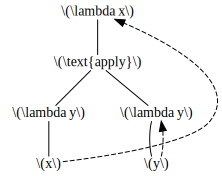
\includegraphics[height=.6\textwidth]{example.png}
                \raisebox{.3\textwidth}{$\rightarrow$}
                \includegraphics[height=.6\textwidth]{example_002.png}

                \includegraphics[width=\textwidth]{framework_003.png}
            \end{center}
        \end{block}
    \end{columns}
\end{frame}


\begin{frame}{Iteracyjne drążenie tematu}
    \begin{columns}
        \column{.5\textwidth}
        \begin{block}{}
            \begin{center}
                \includegraphics[width=\textwidth]{framework_006.png}
            \end{center}
        \end{block}

        \column{.5\textwidth}
        \begin{block}{}
            \begin{center}
                \includegraphics[height=.6\textwidth]{example_004.png}
                \raisebox{.3\textwidth}{$\rightarrow$}
                \includegraphics[height=.6\textwidth]{example_003.png}

                \includegraphics[width=\textwidth]{framework_005.png}
            \end{center}
        \end{block}
    \end{columns}
\end{frame}


\begin{frame}{Iteracyjne drążenie tematu}
    \begin{columns}
        \column{.5\textwidth}
        \begin{block}{}
            \begin{center}
                \includegraphics[width=\textwidth]{framework_007.png}
            \end{center}
        \end{block}

        \column{.5\textwidth}
        \begin{block}{}
            \begin{center}
                \includegraphics[height=.6\textwidth]{example_006.png}
                \raisebox{.3\textwidth}{$\rightarrow$}
                \includegraphics[height=.6\textwidth]{example_005.png}

                \includegraphics[width=.8\textwidth]{framework_008.png}
            \end{center}
        \end{block}
    \end{columns}
\end{frame}


\begin{frame}{Iteracyjne drążenie tematu}
    \begin{block}{}
        \begin{center}
            \includegraphics[width=\textwidth]{framework_009.png}
        \end{center}
    \end{block}
\end{frame}

\begin{frame}{Iteracyjne drążenie tematu}
    \begin{block}{}
        \begin{center}
            \includegraphics[width=\textwidth]{framework_011.png}
        \end{center}
    \end{block}
\end{frame}

\begin{frame}{Iteracyjne drążenie tematu: dalsze prace}
    \begin{block}{}
        \begin{center}
            \includegraphics[width=\textwidth]{framework_011.png}
        \end{center}
    \end{block}
\end{frame}

\begin{frame}{Iteracyjne drążenie tematu: dalsze prace}
    \begin{columns}
        \column{.5\textwidth}
        \begin{block}{}
            \begin{center}
                \includegraphics[width=\textwidth]{framework_012.png}
            \end{center}
        \end{block}

        \column{.5\textwidth}
        \begin{block}{}
            \begin{center}
                \includegraphics[width=\textwidth]{framework_014.png}
            \end{center}
        \end{block}
    \end{columns}
\end{frame}


\section*{}

\begin{frame}{Pytania}
\end{frame}

\end{document}
